\documentclass[8pt]{beamer}

\usetheme{Copenhagen}
\usecolortheme{beaver}
\usepackage[small,center]{caption}
\usepackage{times}
\usefonttheme{structurebold}
\usepackage[english]{babel}
\usepackage{pgf,pgfarrows,pgfnodes,pgfautomata,pgfheaps}
\usepackage{amsmath,amssymb}
\usepackage{amsxtra}

\usepackage{caption}
\usepackage{tikz}
\usetikzlibrary{shapes.misc}

\newcommand{\leftd}[1]{{\color{red} \bar{#1}}}
\newcommand{\interface}[2]{{\color{blue}{#1}_I(#2)}}
\newcommand{\leftdd}[2]{{\color{red} \bar{#1}(\bar{#2})}}
\newcommand{\leftFourier}[1]{{\color{red} \hat{#1}}}
\newcommand{\leftFourierTwo}[2]{{\color{red} \hat{#1}(\hat{#2})}}
\newcommand{\half}{\dfrac{1}{2}}
\newcommand{\divergence}{\mathrm{div}}

\newcommand{\I}{I}

\newcommand*{\vcenterimage}[1]{\vcenter{\hbox{\includegraphics[width=2in]{#1}}}}
\newcommand*{\vcenterarrow}{\vcenter{\hbox{$\Longrightarrow$}}}

\DeclareMathOperator{\hyphen}{-}

\definecolor{RPIred}{rgb}{ 0.87,0.12, 0.20}
\definecolor{ballblue}{rgb}{0.13, 0.67, 0.8}
\definecolor{lightgray}{rgb}{0.83, 0.83, 0.83}
\setbeamercolor{block title}{bg=lightgray,fg=RPIred}
\setbeamercolor{block body}{bg=white,fg=black}
\setbeamercovered{dynamic}
\setbeamercolor*{item}{fg=RPIred}

\captionsetup[subfigure]{labelformat=empty}
\captionsetup[figure]{labelformat=empty}
\setbeamertemplate{navigation symbols}{}
\setbeamertemplate{footline}[frame number]
\begin{document}

% tikz stuff
\tikzset{cross/.style={cross out, draw=black, minimum size=2*(#1-\pgflinewidth),
inner sep=0pt, outer sep=0pt},
%default radius will be 1pt.
cross/.default={2.5pt}}



\frame{
\title{\Large Using \(p\)-Refinement to Increase Boundary Derivative Convergence Rates}

\author{{\Large David Wells \\\vspace{0.1in} Rensselaer Polytechnic Institute}\\
\vspace{0.2in} {In collaboration with:\\{}F. Li, J. W. Banks}}

\date{November 7, 2017\\{} RTG Seminar}

\begin{figure}[h]
\centering
\includegraphics[width=1.5in]{RPI_letterhead.pdf}
 \end{figure}%

\vspace{-0.2in}
\titlepage
}

\section{Goals}
    \begin{frame}
        \frametitle{Goals}
        \begin{itemize}
            \item Efficient numerical methods for elliptic PDEs
            \item Increased accuracy in (normal) boundary derivatives
            \item Improve accuracy in the solution itself; no postprocessing
            \item Order \(n\) data should lead to order \(n\) derivatives
        \end{itemize}
    \end{frame}

\section{A Little on Finite Elements}
\begin{frame}
    \frametitle{Model Problem}
    We will look at linear elliptic problems:
    \begin{equation*}
        -\Delta u + \vec{b} \cdot \nabla u + c u = f
    \end{equation*}
    where \(\mathrm{Re}(c) > 0\) and \(\mathrm{Im}(c)\) may be nonzero.

    \pause
    \vspace{0.5in}
    Let \(X\) be a complete Hilbert space of weakly differentiable
    functions. Find \(u \in X\) such that, for all \(\varphi \in X\)
    \begin{equation*}
        \int_\Omega \nabla u \cdot \nabla \bar{\varphi}
        + \vec{b} \cdot \nabla u \bar{\varphi}
        + c u \bar{\varphi}
        dx
        =
        \int_\Omega f \bar{\varphi} dx
    \end{equation*}
    If \(X\) is finite dimensional then we have a numerical method.
\end{frame}

\begin{frame}
    \frametitle{The Finite Element Method}
    \begin{figure}
        \centering
        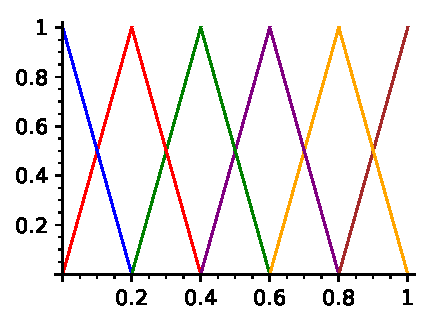
\includegraphics[width=3in]{fe-basis.pdf}

        We usually use piecewise polynomials as a basis.
    \end{figure}
\end{frame}

\begin{frame}
    \frametitle{The Finite Element Method}
    \begin{figure}
        \centering
        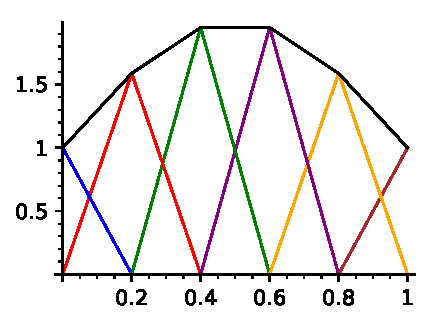
\includegraphics[width=3in]{fe-interpolation.pdf}

        The solution (in black) is some linear combination of the basis.
    \end{figure}
\end{frame}

\begin{frame}
    \frametitle{The Finite Element Method}

    \begin{figure}
        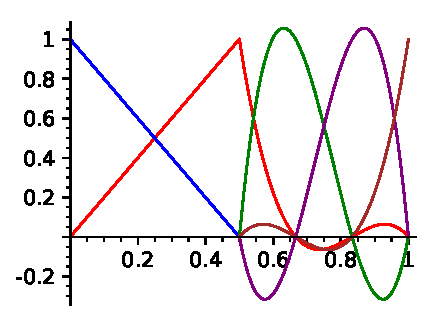
\includegraphics[width=3in]{p-refinement.pdf}

        Example of \(p\)-refinement in 1D: a linear cell next to a cubic cell.
    \end{figure}
\end{frame}

\begin{frame}
    \frametitle{The Finite Element Method}

    \begin{figure}
        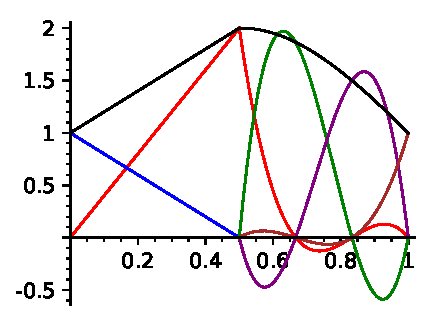
\includegraphics[width=3in]{p-refinement-interpolate.pdf}

        The solution (in black) as a linear combination of the basis.
    \end{figure}
\end{frame}

\section{Superconvergence}
\begin{frame}
    \frametitle{Assumptions}
    \begin{itemize}
        \item Linear, constant coefficient elliptic PDEs, Dirichlet (or
              periodic) boundary conditions
              \pause
        \item \emph{Lots} of regularity
              \pause
        \item Uniform grid (constant \(\Delta x\), \(\Delta y\)) of tensor
              product elements (no triangles)
              \pause
        \item Continuous finite element spaces
              \begin{itemize}
                  \item in 1D, degree \(n\) on interior elements, degree \(n +
                        p\) on nonperiodic edge elements
                  \item in 2D, bilinear on interior elements, degree \(1 \otimes
                        1 + p\) on nonperiodic edge elements
              \end{itemize}
    \end{itemize}
\end{frame}

\begin{frame}
    \frametitle{What's the plan?}
    \begin{itemize}
        \item Static \(p\)-refinement: some cells have higher degree polynomial bases
        \item Global \(h\)-refinement: no mesh adaptivity (yet)
        \item Not really an \(hp\)-element method, but similar
    \end{itemize}
\end{frame}

\begin{frame}
    \frametitle{What's the plan?}
    \begin{center}
        Picking the right type of \(p\)-refinement improves the boundary
        derivative convergence rates.
    \end{center}
\end{frame}

\begin{frame}
    \frametitle{Superconvergence in 1D}
    Classic idea based on Greens' functions (Arnold et al, 1974):
    \begin{equation*}
        -u_{xx} + b u_x + c u = f \Leftrightarrow
        a(u, \varphi) = (f, \varphi)
    \end{equation*}
    \pause

    Suppose \(u \in X\) and \(u^h \in X^h \subset X\).
    \begin{align*}
        |u^h(i \Delta x) - u(i \Delta x)|
        &= |a(G_{i\Delta x}, u^h - u)|                                        \\
        &= |a(G_{i\Delta x} - v^h, u^h - u)|                                  \\
        &\leq C_1 \|G_{i\Delta x} - v^h\|_{H^1} \|u^h - u\|_{H^1}             \\
        &\leq C_2 \Delta x^{2 k}.
    \end{align*}
\end{frame}

\begin{frame}
    \frametitle{Superconvergence in 1D}
    \begin{figure}
        \centering

        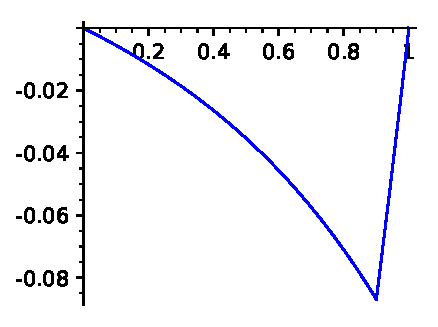
\includegraphics[width=3in]{greens-cdr.pdf}

        Plot of the Greens' function centered at \(1 - \Delta x\) with ten cells.
    \end{figure}
\end{frame}

\begin{frame}
    \frametitle{Superconvergence in 1D}
    Greens' functions centered near the boundary scale like \(O(\Delta x)\). We
    can exploit this to gain an order of convergence:
    \begin{theorem}[Wells, Li, Banks, 2017]
        Suppose that the finite element space consists of piecewise order \(k\)
        polynomials on non-boundary cells and order \(k + 1\) polynomials on
        boundary cells. Then
        \begin{equation*}
            |u(L - \Delta x) - u^h(L - \Delta x)|
            \leq
            \dfrac{\gamma}{\sqrt{\alpha}} |D|^{k + 1} \sqrt{C_1}
            \|u\|_{W^{k + 1,\infty}} \Delta x^{2 k + 1}
        \end{equation*}
        which is one order higher than the standard interior rate. \(D,
        \gamma\), \(\alpha\), and \(C_1\) are constants dependent on \(b, c\),
        and \(k\).
    \end{theorem}

    \begin{proof}
        With constant \(b\) and \(c\) we can write down a closed formula for the
        Greens' function and bound its derivatives with standard inequalities.
    \end{proof}
\end{frame}

\begin{frame}
    \frametitle{Improving boundary derivative convergence in 1D}
    The error has two components:
    \begin{itemize}
        \item Error from coupling to the rest of the domain (last result)
        \item Error in the local approximation space
    \end{itemize}
    \pause

    \begin{theorem}[Wells, Li, Banks, 2017]
        Consider a finite element discretization with cells of order \(k\)
        on the interior and cells of order \(k + p\) on the boundary. Then
        \begin{align*}
            \left\|
            \dfrac{d^n}{dx^n}\left(u - u^h\right)
            \right\|_{L^\infty([L - \Delta x, L])}
            \nonumber
            &\leq
            C_2 |D|^{2 k + p + 3} \max\left(2, \dfrac{1}{|D|\Delta x}\right)
            \dfrac{\gamma^3}{\alpha^{3/2}}
            \|u^{(k + 1)}\|_{L^\infty} \Delta x^{2 k + 1}                     \\
            &\phantom{\leq}
            +
            C_3
            D^2 \dfrac{\gamma^2}{\alpha}
            \|u(x)\|_{W^{k + p + 1, \infty}}
            \Delta x^{k + p - n + 1}
        \end{align*}
    \end{theorem}

    \begin{proof}
        Use the decomposition of the error to control each part.
    \end{proof}
\end{frame}

\begin{frame}
    \frametitle{Improving boundary derivative convergence in 1D}
    If we combine constants independent of \(u\):
    \begin{equation*}
        \left\|\dfrac{d^n}{dx^n}(u - u^h)\right\|_{L^\infty([L - \Delta x, L])}
        \leq
        C
        \left(
        \|u^{(k + 1)}(x)\|_{L^\infty}
        \Delta x^{2 k}
        +
        \|u(x)\|_{L^\infty} \Delta x^{k + p - n + 1}
        \right)
    \end{equation*}

    For cubic elements on the boundary and linear elements everywhere else we
    can get a second-order accurate second derivative at the boundary.
\end{frame}

\begin{frame}
    \frametitle{Numerical Results}
    Domain of \([0, 1]\), with manufactured solution
    \begin{equation*}
        u = \sin(10 x)
    \end{equation*}
    \begin{itemize}
        \item Use \texttt{deal.II}'s \(hp\)-finite element support
        \item Bulk order \(2\), boundary orders \(2\), \(3\), and \(4\)
        \item CDR equation
        \item Solve with GMRES
    \end{itemize}
\end{frame}

\begin{frame}
    \frametitle{Numerical Results}
    \begin{figure}
        \centering
        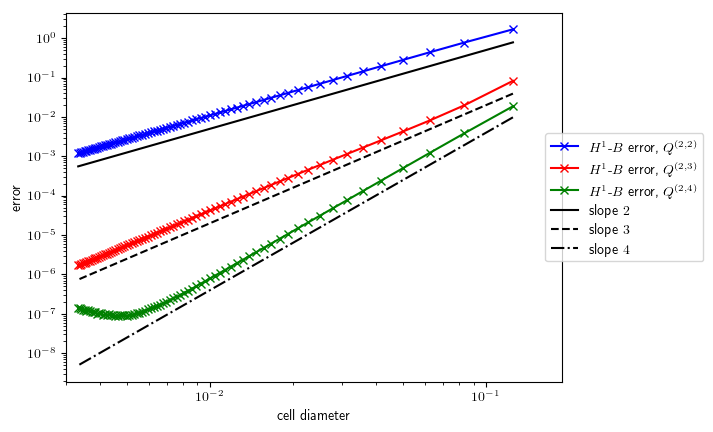
\includegraphics[width=4in]{Pictures/oned-cdr-2-h1-errors.png}

        \caption{Convergence rates for the \(p\)-refinement scheme of the
        first derivative on the boundary. We hit roundoff error near the end.}
    \end{figure}
\end{frame}

\begin{frame}
    \frametitle{Numerical Results}
    \begin{figure}
        \centering
        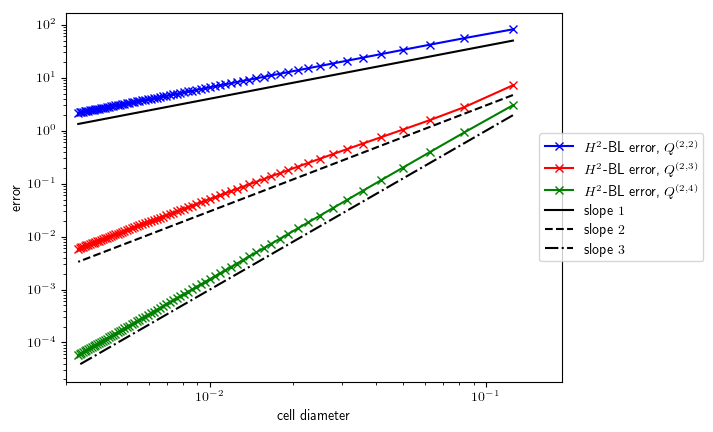
\includegraphics[width=4in]{Pictures/oned-cdr-2-h2-errors.png}

        \caption{Convergence rates for the \(p\)-refinement scheme of the second
        derivative on the boundary.}
    \end{figure}
\end{frame}

\section{\(p\)-refinement in 2D}
    \begin{frame}
        \frametitle{Extension to 2D}
        Greens' functions are not nearly as useful in 2D, but they give us the
        fundamental tool we need.

        Suppose that our domain is periodic in the \(x\)-direction. We can
        extend the 1D analysis by using a discrete analog of the Fourier
        transform:
        \begin{equation*}
            X = V^{\Delta x} \otimes V^{\Delta y},
            v \in X \Rightarrow
            v = \sum_{i,j} c_{ij} F_i(x) Y_j(y)
        \end{equation*}
        where \(F_i(x)\) is a linear interpolant of the \(i\)th Fourier mode.
    \end{frame}

    \begin{frame}
        \frametitle{Extension to 2D}
        \begin{center}
            \(\{F_k(x)\}\) is a basis for \(V^{\Delta x}\) which decouples the
            \emph{discretization} into multiple one-dimensional problems.
        \end{center}
    \end{frame}

    \begin{frame}
        \frametitle{Extension to 2D}
        Suppose that our domain is \([0, 1] \times [0, L]\):
        \begin{equation*}
            u^h(x, y) = \sum_{k = 0}^{N - 1} F_k(x) \hat{u}^h_k(y) :
            F_k(x) \in V^{\Delta x},
            \hat{u}^h(y) \in V^{\Delta y}.
        \end{equation*}
        \pause
        \begin{equation*}
            \int_0^L
            \hat{u}^h_{k, y} \bar{\phi}_y
            + b_1 \hat{u}_{k, y} \bar{\phi}
            + \dfrac{\lambda_{A, k}}{\lambda_{M, k}}
            \hat{u}^h_k \bar{\phi} dy
            =
            \int_0^L
            \left(
            \int_0^1
            \dfrac{f(x, y) F_k(x)}{\lambda_{M, k}} dx
            \right)
            \bar{\phi} dy,
            \forall \phi(y) \in V^{\Delta y}.
        \end{equation*}
        Here \(\lambda_{M,k}\) and \(\lambda_{A,k}\) are eigenvalues of the
        (circulant) 1D mass and stiffness matrices.
        \pause
        \vspace{0.25in}

        The 1D result applies to each \(\hat{u}^h_k(y)\), implying normal
        derivative superconvergence at mesh knots.
    \end{frame}

    \begin{frame}
        \begin{theorem}
            Consider a tensor-product discretization of the CDR equation with
            linear elements in the periodic (\(x\)) direction, \(Q^1\) elements
            on the interior, and \(Q^{(1, 1 + p)}\) elements on the Dirichlet
            boundary. If \(f\) and \(u\) are sufficiently smooth then for
            constants \(C_3\) and \(C_4\) dependent data
            \begin{equation*}
                \left|
                \dfrac{d^n}{dy^n}
                \left(u(x, y) - u^h(x, y) \right)
                \bigg|_{(\delta_i, \delta_{N^*})}
                \right|
                \leq
                C_3 \Delta x^2
                +
                C_4 (\Delta y^2 + \Delta y^{2 + p - n})
            \end{equation*}
            where \(N^* = 0\) or \(N^* = N\).

            \begin{proof}
                Use the Fourier series of \(u\) and \(f\) and use a triangle
                inequality argument between \(u\), \(u^h\), and a
                semidiscretization (continuous in \(x\)) solution to the weak
                equation.
            \end{proof}
        \end{theorem}
    \end{frame}

\begin{frame}
    \frametitle{Numerical Results}
    Manufactured solution with \(\vec{b} = (1, 1)\) and \(c = 2\):
    \begin{equation*}
        u(x, y) = (y^3 + \exp(-y^2) + \sin(4.5 y^2) + \sin(20 y)) (20 \cos(4 \pi x)
        + 0.1 \sin(20 \pi x) - 80 \sin(6 \pi x))
    \end{equation*}
    \pause
    \(H^1{\hyphen}B\) error defined as
    \begin{equation*}
        \max_{i, j}
        \left|
        (\nabla u^h \cdot \vec{n} -
        \nabla u \cdot \vec{n})(\delta_i, \delta_j)
        : (\delta_i, \delta_j) \in \partial \Omega^h
        \right|
    \end{equation*}
    and \(H^2{\hyphen}B\) error defined as
    \begin{equation*}
        \max_{i, j}
        \left|
        (\vec{n}^T \Delta u^h \cdot \vec{n} -
        \vec{n}^T \Delta u \cdot \vec{n})(\delta_i, \delta_j)
        : (\delta_i, \delta_j) \in \partial \Omega^h
        \right|.
    \end{equation*}
\end{frame}

\begin{frame}
    \frametitle{Numerical Results}
    \begin{figure}
        \centering
        Elimination of nonnormal \(p\)-refinement:
        \begin{tikzpicture}[scale=1.5]
    %% leftmost pair
    % cubic square
    \draw[-, thick] (-1.0, 0.0) -- (-1.0, 1.0);
    \draw[-, thick] (0.0, 0.0) -- (0.0, 1.0);
    \draw[-, thick] (-1.0, 0.0) -- (0.0, 0.0);
    \draw[-, thick] (-1.0, 1.0) -- (0.0, 1.0);

    % linear square
    \draw[-, thick] (-1.0, -1.0) -- (-1.0, 0.0);
    \draw[-, thick] (0.0, -1.0) -- (0.0, 0.0);
    \draw[-, thick] (-1.0, -1.0) -- (0.0, -1.0);
    \draw[-, thick] (-1.0, 0.0) -- (0.0, 0.0);

    % cubic support points
    \foreach \x in {0,...,4}
    \foreach \y in {0,...,4}
        \draw (0.25*\x - 1.0, 0.25*\y) node[cross] {};

    % linear support points
    \foreach \x in {0,...,1}
    \foreach \y in {0,...,1}
        \draw (\x - 1.0, \y - 1.0) circle (2pt);

    %% second pair
    % cubic square
    \draw[-, thick] (0.0, 0.0) -- (0.0, 1.0);
    \draw[-, thick] (1.0, 0.0) -- (1.0, 1.0);
    \draw[-, thick] (0.0, 0.0) -- (1.0, 0.0);
    \draw[-, thick] (0.0, 1.0) -- (1.0, 1.0);

    % linear square
    \draw[-, thick] (0.0, -1.0) -- (0.0, 0.0);
    \draw[-, thick] (1.0, -1.0) -- (1.0, 0.0);
    \draw[-, thick] (0.0, -1.0) -- (1.0, -1.0);
    \draw[-, thick] (0.0, 0.0) -- (1.0, 0.0);

    % cubic support points
    \foreach \x in {0,...,4}
    \foreach \y in {0,...,4}
        \draw (0.25*\x, 0.25*\y) node[cross] {};

    % linear support points
    \foreach \x in {0,...,1}
    \foreach \y in {0,...,1}
        \draw (\x, \y - 1.0) circle (2pt);

    \draw[->, thick] (1.5, 0.0) -- (2.5, 0.0);

    % cubic square
    \draw[-, thick] (3.0, 0.0) -- (3.0, 1.0);
    \draw[-, thick] (4.0, 0.0) -- (4.0, 1.0);
    \draw[-, thick] (3.0, 0.0) -- (4.0, 0.0);
    \draw[-, thick] (3.0, 1.0) -- (4.0, 1.0);

    % linear square
    \draw[-, thick] (3.0, -1.0) -- (3.0, 0.0);
    \draw[-, thick] (4.0, -1.0) -- (4.0, 0.0);
    \draw[-, thick] (3.0, -1.0) -- (4.0, -1.0);
    \draw[-, thick] (3.0, 0.0)  -- (4.0, 0.0);

    % cubic support points
    \foreach \x in {0,...,1}
    \foreach \y in {0,...,4}
        \draw (3.0 + \x, 0.25*\y) node[cross] {};

    % linear support points
    \foreach \x in {0,...,1}
    \foreach \y in {0,...,1}
        \draw (3.0 + \x, \y - 1.0) circle (2pt);

    %% rightmost pair
    % cubic square
    \draw[-, thick] (4.0, 0.0) -- (4.0, 1.0);
    \draw[-, thick] (5.0, 0.0) -- (5.0, 1.0);
    \draw[-, thick] (4.0, 0.0) -- (5.0, 0.0);
    \draw[-, thick] (4.0, 1.0) -- (5.0, 1.0);

    % linear square
    \draw[-, thick] (4.0, -1.0) -- (4.0, 0.0);
    \draw[-, thick] (5.0, -1.0) -- (5.0, 0.0);
    \draw[-, thick] (4.0, -1.0) -- (5.0, -1.0);
    \draw[-, thick] (4.0, 0.0)  -- (5.0, 0.0);

    % cubic support points
    \foreach \x in {0,...,1}
    \foreach \y in {0,...,4}
        \draw (4.0 + \x, 0.25*\y) node[cross] {};

    % linear support points
    \foreach \x in {0,...,1}
    \foreach \y in {0,...,1}
        \draw (4.0 + \x, \y - 1.0) circle (2pt);
\end{tikzpicture}

        \caption{Depiction of normal \(p\)-refinement scheme, with elimination
        of extra DoFs. Linear DoFs are circles, quartic are crosses.}
    \end{figure}
\end{frame}

\begin{frame}
    \frametitle{Numerical Results}
    \begin{figure}
        \centering
        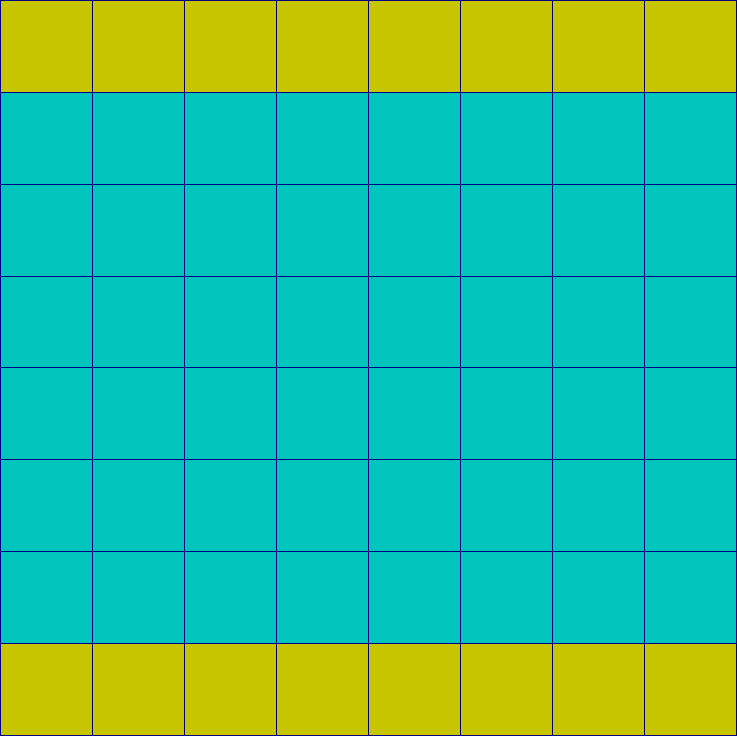
\includegraphics[width=2.5in]{Pictures/square-periodic-grid.png}

        \caption{Depiction of the square grid with bulk cells in cyan and
        \(p\)-refined cells in yellow.}
    \end{figure}
\end{frame}

\begin{frame}
    \frametitle{Numerical Results}
    \begin{figure}
        \centering
        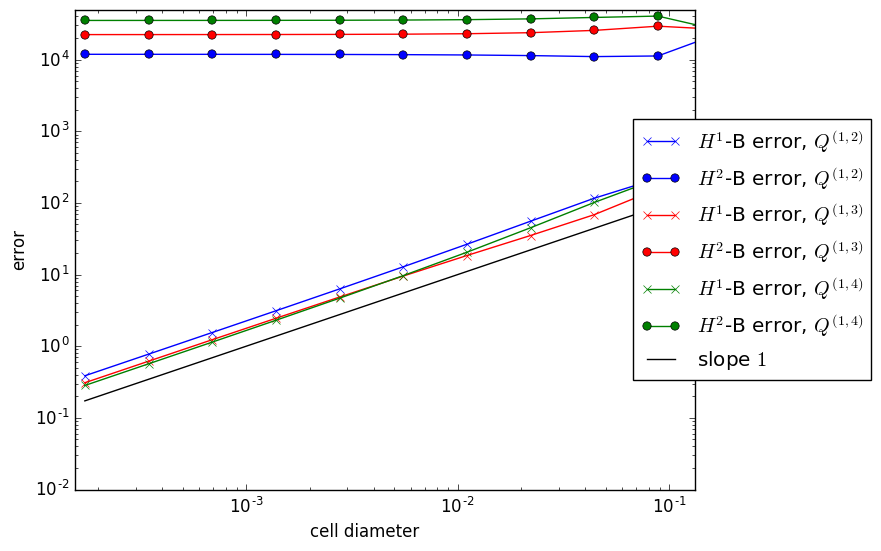
\includegraphics[width=3in]{Pictures/periodic-dont-eliminate-nonnormal-convergence.png}

        \caption{Convergence rates with anisotropic \(p\)-refinement. We do not
        recover any higher order accurate derivatives.}
    \end{figure}
\end{frame}

\begin{frame}
    \frametitle{Numerical Results}
    \begin{figure}
        \centering

        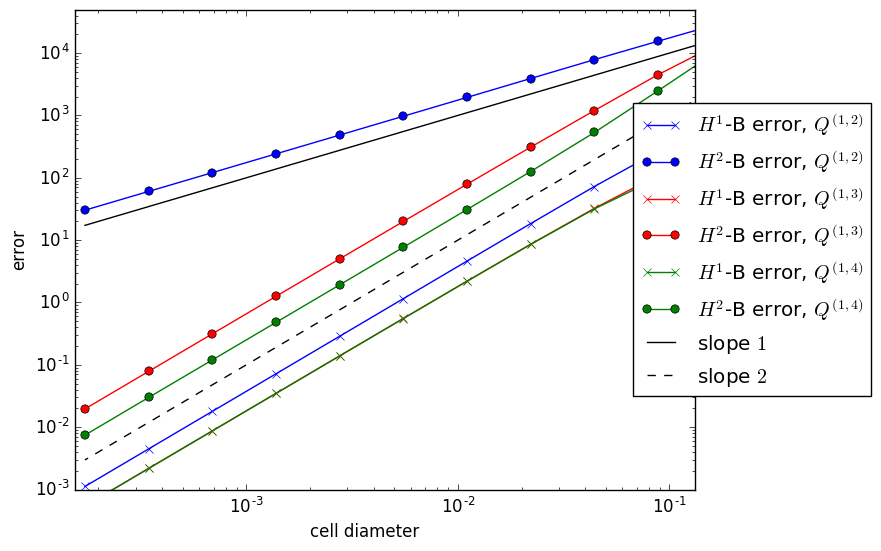
\includegraphics[width=3in]{Pictures/periodic-nonnormal-convergence.png}

        \caption{Convergence rates with isotropic \(p\)-refinement. The 1D
        theory applies at the knots.}
    \end{figure}
\end{frame}

\begin{frame}
    \frametitle{Numerical Results}
    \begin{figure}
        \centering

        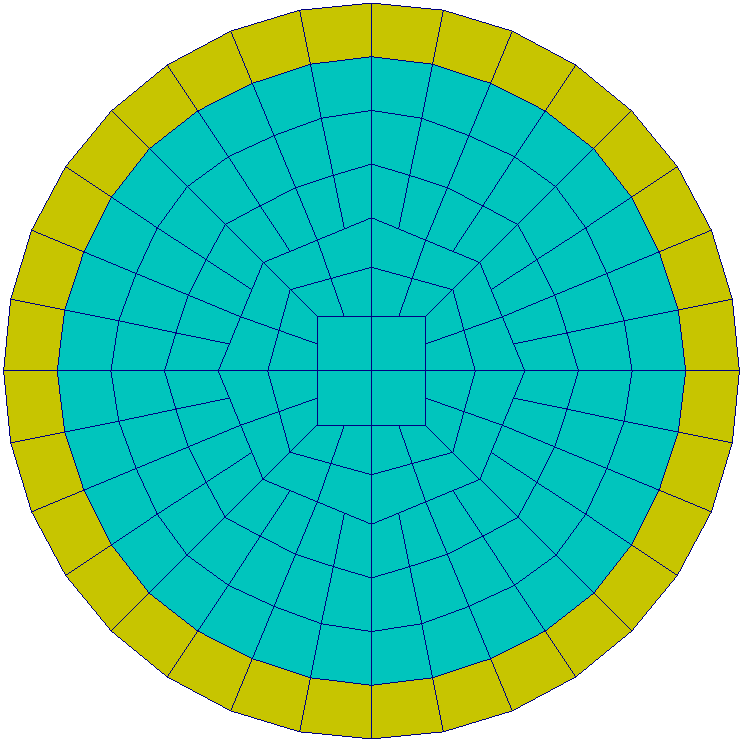
\includegraphics[width=2.5in]{Pictures/circular-grid.png}
        \caption{A circular grid with a geometry described near the boundary in
        polar coordinates, in the middle with Cartesian coordinates, and a
        transfinite interpolation in-between.}
    \end{figure}
\end{frame}

\begin{frame}
    \frametitle{Numerical Results}
    \begin{figure}
        \centering

        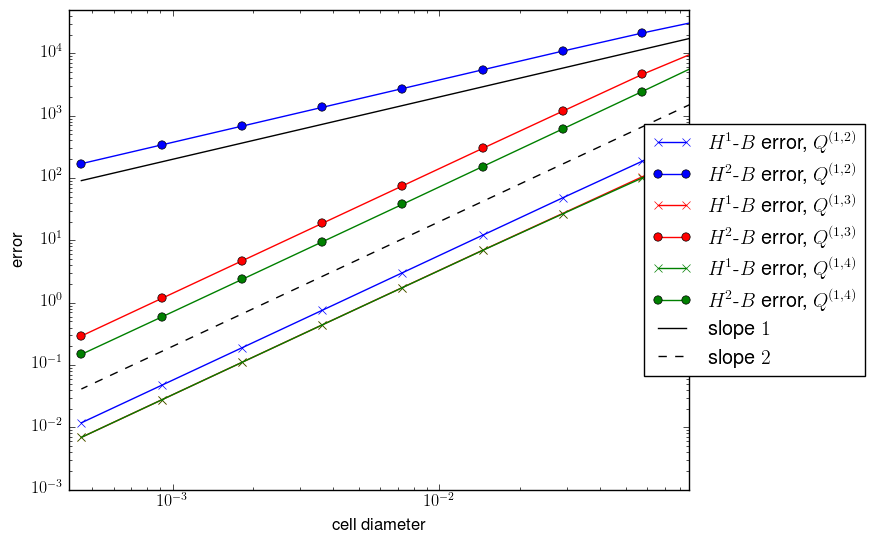
\includegraphics[width=3in]{Pictures/circle-nonnormal-convergence.png}
        \caption{Rates of convergence for the circular grid.}
    \end{figure}
\end{frame}

\section{Summary}
\begin{frame}
    \frametitle{Summary and Outlook}
    \begin{itemize}
        \item \(p\)-refinement error estimates involve a coupling term and a
              local term
        \item We can achieve higher-order derivative approximation at isolated
              points
        \item Future work: escape the Fourier framework, higher-order bulk
              elements, better tools for describing arbitrary geometries
    \end{itemize}

    \vspace{0.5in}
    \begin{center}
        \textcolor{RPIred}{\Huge Thank You!}
    \end{center}
\end{frame}

\end{document}
